\documentclass{article}
\usepackage[utf8]{inputenc}
\usepackage{graphicx}
\usepackage{hyperref}
\usepackage{xcolor}
\usepackage{multirow}
\usepackage{float}

\title{\textbf{Stock Price and Direction Prediction via Deep Attention-Based Convolutional Neural Networks}}
\author{Onur Alaçam, Tuğcan Hoşer, Uygar Kaya, Tuna Tuncer}
\date{\textbf{2022 Spring}}

\begin{document}

\begin{figure}[h]
    \begin{center}
        
\includegraphics[]{assets/OzU.png}
    \end{center}
\end{figure}

\begin{center}
    OZYEGIN UNIVERSITY\\*
    FACULTY OF ENGINEERING\\*
    DEPARTMENT OF COMPUTER SCIENCE
\end{center}

\begin{center}
    \textbf{CS 402}\\* \vspace{0.2cm}
    \textbf{2022 Spring}\\* \vspace{0.4cm}
    \textbf{SENIOR PROJECT REPORT}\\* \vspace{0.6cm}
    \textbf{Stock Price and Direction Prediction via Deep Attention-Based Convolutional Neural Networks}\\* \vspace{0.8cm}
    \textbf{By}\\*
    \textbf{Onur Alaçam, Tuğcan Hoşer, Uygar Kaya, Tuna Tuncer}\\* \vspace{0.6cm}
    \textbf{Supervised By}\\*
    \textbf{Assistant Prof. Emre Sefer}\\* \vspace{0.6cm}
\end{center}
\textbf{Declaration of Own Work Statement/ (Plagiarism Statement)}\\*
Hereby I confirm that all this work is original and my own. I have clearly referenced/listed all sources as appropriate and given the sources of all pictures, data etc. that are not my own. I have not made any use of the essay(s) or other work of any other student(s) either past or present, at this or any other educational institution. I also declare that this project has not previously been submitted for assessment in any other course, degree or qualification at this or any other educational institution.\vspace{0.2cm}\\*
\textbf{Student Name and Surname:}\\* Onur Alaçam, Tuğcan Hoşer, Uygar Kaya, Tuna Tuncer \vspace{0.1cm}\\*
\textbf{Signature:} \vspace{0.9cm}\\*
\textbf{Place, Date:}\\* Istanbul, Turkey - 27.05.2022

\tableofcontents

\maketitle
\begin{center}
    \textbf{\Large Abstract}
\end{center}
Since stock prices are time series data, most academic studies have focused on time series forecasting in machine learning models. Unfortunately, these models do not perform as well as excepted. In this project, we converted the 1-D time-series data to 2-D images with the help of the technical indicators. Then, using these images, we compared a few state-of-the-art models in the field of computer vision such as ConvMixer, Vision Transformer, MLP-Mixer and the CNN-TA model, which is also used for predicting stock prices in the literature before. We investigated the effects of self-attention and patch embedding in the finance area. Implementations of all models are done in Tensorflow - Keras framework in the Python Programming Language.


\begin{center}
    \section{Introduction}
\end{center}
In the last decade, Machine Learning architectures have started to become popular in finance as in other fields, however, most of these architectures do not give the expected performance in the time series data with current technologies. Thus, Deep Learning architectures have recently attracted more attention. Specifically, in recent years, with the discovery of the attention mechanism, there have been crucial developments in the field of Computer Vision, hence we decided to apply this potential to the field of finance. In order to take advantage of Computer Vision models, we had to convert the time series data into images. \vspace{0.0005cm} \\*
In our research, we use the Vision Transformer architecture, which uses patch embedding and applies the attention mechanism to transformer models, and the ConvMixer architecture, which integrates the patch embeddings structure into Convolutional Neural Networks. Also, in our project, we have implemented the main architecture of the article "Algorithmic Financial Trading with Deep \textbf{Convolutional Neural Networks}"[2], in order to compare the results we will get from these architectures. \vspace{0.2cm} \\*
It's a fact for many years that the convolutional neural networks has dominated the computer vision field, but the Vision Transformer claims to outperform CNNs in most cases. It is believed that patch embedding, and self-attention mechanisms, and the complex transformer structure are crucial parts of the success of Vision Transformer. On the other hand, ConvMixer, which was released in January 2022, is claiming to perform better than both Vision Transformer and other CNN models. Moreover, the authors of the ConvMixer, claim that the success of the Vision Transformer is the result of the patch embedding mechanism rather than the complex transformer architecture of the model. Our aim is to show the effects of both patch embedding and self-attention mechanisms on the finance field by comparing these architectures. \vspace{0.2cm} \\*
As we mentioned above, we used technical indicators to obtain images from time series data for the project, each row of our images represents a different day, while each column represents a different technical indicator value. Since we used 67 different technical indicators in total, the size of our images became 67x67. By putting these images into the 3 different architectures, ConvMixer, Convolutional Neural Network, and Vision Transformer, we compared each of our models in terms of Computational Model Performance and Financial Evaluation. \vspace{0.2cm} \\*
The background will be covered in the second chapter, where we will discuss the approaches, tools, and technology that we have used in our senior project. The third chapter will discuss our problem statement and the problem we are attempting to solve. The fourth chapter will describe how we tackled the problem and how we came up with answers. In the fifth chapter, we will be examining our findings and what we were able to accomplish, and what we were unable to accomplish. We've mentioned flaws we found when looking at the outcomes in the findings, as well as how we might fix them in the future. We compare our technique and model to other comparable works in the sixth chapter. The seventh chapter contains our conclusion as well as our recommendations.

\begin{center}
    \item\section{Background}
\end{center}
In this project, many different techniques, methods, tools, data and indicators were used.\vspace{0.25cm} \\*
\textbf{Nvidia CUDA:} Nvidia Cuda is a set of development tools that enable algorithms to run on the GPU. We used Nvidia Cuda with PyTorch to train the model faster.\vspace{0.1cm}\\*
\textbf{S\&P:} The S\&P 500 includes major American companies. It covers about 75\% of the American stock market. We used data from the last 20 years of S\&P.\vspace{0.1cm}\\*
\textbf{Yahoo Finance:} Yahoo Finance provides financial news, data and commentary including stock quotes, press releases, financial reports, and original content. We downloaded the S\&P 500 dataset from here. In addition, we will consider companies individually in the future and we plan to download their data from Yahoo Finance.\vspace{0.1cm}\\*
\textbf{Pandas:} Pandas is a software library written in the Python programming language for data manipulation and analysis. We processed numerical data and tables with using this library.\vspace{0.1cm}\\*
\textbf{Numpy:} NumPy is a library for the Python programming language that supports large, multidimensional arrays and matrices, adding high-level mathematical functions to operate on these arrays.\vspace{0.1cm}\\*
\textbf{TA-Lib:} TA-Lib is a library that contains 150 different indicators, especially used for trading algorithms. We also used 11 different indicators thanks to this library.\vspace{0.1cm}\\*
\textbf{TensorFlow:} TensorFlow is a free \& open source software library for machine learning. The architectures in the articles we compared used TensorFlow because they were implemented in TensorFlow.\vspace{0.1cm}\\*
\textbf{Keras:} Keras is an open source neural network library written in Python. Our architectures are implemented using Keras.\vspace{0.1cm}\\*
\textbf{Sklearn:} Scikit-learn is a free software machine learning library for the Python programming language. It is used to separate data, scale, and measure metrics as a result of the architecture.\vspace{0.1cm}\\*
\textbf{Matplotlib:} Matplotlib is a plotting library for the Python programming language and numerical math extension NumPy. We used it to visualize the results from our data.\vspace{0.5cm}\\*
\textbf{\large Indicators} \vspace{0.1cm}\\*
We got the data of S\&P 500 from Yahoo Finance from 2001 to 2021. We have turned these data into pictures by adhering to 11 economic technical indicators. In this part, we will talk about the indicators we have used.\vspace{0.3cm}\\*
\textbf{RSI: Relative Strength Index}\\*
The Relative Strength Index (RSI) is an indicator that provides predictions about the direction of the short and medium-term trend calculated by comparing the closing values of the relevant period with the previous closing values of the period.
\begin{figure}[H]
\begin{center}
   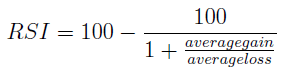
\includegraphics[width=55mm,scale=0.5]{assets/formulas/rsi.png}
   \caption{RSI Formula}
\end{center}
\end{figure}
\noindent
\textbf{WMA: Weighted Moving Average} \\*
A Weighted Moving Average puts more weight on recent data and less on past data. This is done by multiplying each bar’s price by a weighting factor. Because of its unique calculation, WMA will follow prices more closely than a corresponding Simple Moving Average.
\begin{figure}[H]
\begin{center}
   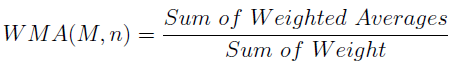
\includegraphics[width=85mm,scale=0.8]{assets/formulas/wma.png}
   \caption{WSI Formula}
\end{center}
\end{figure}
\noindent
\textbf{EMA: Exponential Moving Average} \\*
EMA, which stands for Exponential Moving Average, is used as an indicator of moving averages. Through the EMA, traders can watch exponential moving averages on the charts. By giving weight to last minute data such as EMA closing prices, the time that can progress with the weights assigned to the relevant data is based on the exponentially decreasing process.
\begin{figure}[H]
\begin{center}
   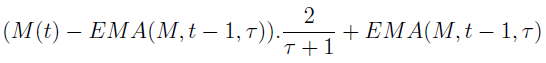
\includegraphics[width=95mm,scale=0.8]{assets/formulas/ema.png}
   \caption{EMA Formula}
\end{center}
\end{figure}
\noindent
\textbf{SMA: Simple Moving Average} \\*
Simple Moving Average (SMA) is the simplest form of moving averages. It is obtained by dividing the total of data by the number of data.
\begin{figure}[H]
\begin{center}
   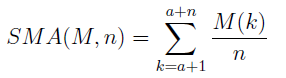
\includegraphics[width=55mm,scale=0.8]{assets/formulas/sma.png}
   \caption{SMA Formula}
\end{center}
\end{figure}
\noindent
\textbf{ROC: Rate of Change}\\*
The Rate of Change Indicator (ROC) is a kind of momentum oscillator. Calculates the rate of price change between periods.
\begin{figure}[H]
\begin{center}
   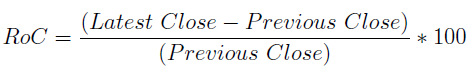
\includegraphics[width=80mm,scale=0.8]{assets/formulas/roc.png}
   \caption{ROC Formula}
\end{center}
\end{figure}
\noindent
\textbf{CMO: Chande Momentum Oscilator Indicator} \\*
The Chande Momentum Oscillator (CMO) is calculated by dividing the sum of the momentum on the up days and the sum of the momentum on the down days by dividing the sum of the momentum on the up days by the sum of the momentum on the down days and multiplying by 100 to make a percentage.
\begin{figure}[H]
\begin{center}
   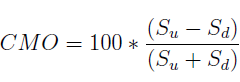
\includegraphics[width=45mm,scale=0.8]{assets/formulas/cmo.png}\\*
   \textit{$S_U$: Total momentum of the up days for the analysis period}\vspace{0.1cm}\\*
   \textit{$S_D$: Total momentum of the down days for the analysis period}\vspace{0.2cm}\\*
   \caption{CMO Formula}
\end{center}
\end{figure}
\noindent
\textbf{CCI: Commodity Channel Index} \\*
Commodity Channel Index (CCI) is an indicator that compares current prices and the average price over a period of time.
\begin{figure}[H]
\begin{center}
   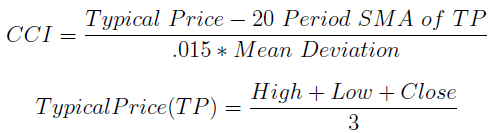
\includegraphics[width=80mm,scale=0.8]{assets/formulas/cci.png}
   \caption{CCI Formula}
\end{center}
\end{figure}
\noindent
\textbf{PPO: Percentage Price Oscillator} \\*
The Percentage Price Oscillator (PPO) is a technical momentum indicator that displays the relationship between two moving averages in percentage terms. The moving averages are the 26-period and 12-period exponential moving average (EMA).
\begin{figure}[H]
\begin{center}
   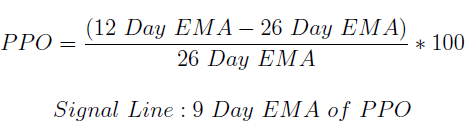
\includegraphics[width=80mm,scale=0.8]{assets/formulas/ppo.png}
   \caption{PPO Formula}
\end{center}
\end{figure}
\noindent
\textbf{TEMA: Triple Exponential Moving Average} \\*
Triple Exponential Moving Average (TEMA) is a type of EMA indicator that provides the reduction of minor price fluctuations and filters out volatility.
\begin{figure}[H]
\begin{center}
   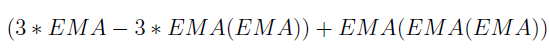
\includegraphics[width=90mm,scale=0.8]{assets/formulas/tema.png}
   \caption{TEMA Formula}
\end{center}
\end{figure}
\noindent
\textbf{WILLR: Williams} \\*
Williams \%R, also known as the Williams Percent Range, is a type of momentum indicator that moves between 0 and -100 and measures overbought and oversold levels.
\begin{figure}[H]
\begin{center}
    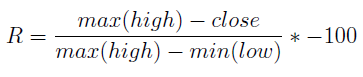
\includegraphics[width=75mm,scale=0.8]{assets/formulas/willr.png}
    \caption{WILLR Formula}
\end{center}
\end{figure}
\noindent
\textbf{MACD: Moving Average Convergence and Divergence} \\*
The Moving Average Convergence and Divergence (MACD) indicator is a technical indicator that displays how stock values are trending.
\begin{figure}[H]
\begin{center}
    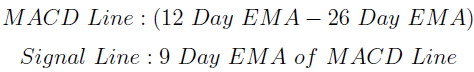
\includegraphics[width=80mm,scale=0.8]{assets/formulas/macd.png}
    \caption{MACD Formula}
\end{center}
\end{figure}
\noindent

\begin{center}
    \item\section{Problem Statement}
\end{center}
It is quite common to convert the image into neural networks and make predictions from it. In our case, it is based on taking financial data and converting them into images with the help of indicators and making predictions on these images. This is a method that has been used before, but our mission here is to show that with whichever model we make these predictions, we will achieve a more successful result. \vspace{0.2cm}\\*
We decided to implement this project with our supervisor Assistant Prof. Emre Sefer to solve this problem. Afterward, we thoroughly researched the issue and discussed the improvements we could make. \vspace{0.0005cm}\\*
While creating the images, it is necessary to choose the technical indicators well and to create the image according to the connection of these indicators with each other. In addition, if the number of data we pull increases, the images will increase, and if we use CPU when we want to train them, it will take a lot of time at high epoch values, so we plan to use Nvidia CUDA.

\begin{center}
    \item\section{Solution Approach}
\end{center}
\subsection{Dataset Preparation}
First and foremost, we had to decide whether we would proceed with our work on stocks or cryptocurrencies.\vspace{0.2cm}\\*
Due to the high volatility of cryptocurrencies, the accuracy of the predictions to be made with the models could be lower. Because, in today's cryptocurrency market, which can change rapidly with the tweets of celebrities, our work could be more challenging. However, once our model for stocks in CS402 is ready, we want to train the same models on cryptocurrencies and compare the outcomes. \vspace{0.01cm} \\*
In the paper \textit{Algorithmic Financial Trading with Deep Convolutional Neural Networks: Time Series to Image Conversion Approach} [2], it was reported that models with ETF data outperformed the models with Dow30 data in terms of accuracy. That's why we chose to use the S\&P500. We also wanted to include the 2008 economic crisis so that our dataset does not exhibit an entirely increasing market trend. As a result, we generated our dataset utilizing data from 2001-10-11 to 2021-11-11.\vspace{0.1cm}\\*
After we created our dataset, we converted it into images to use in our architectures. We constructed our images by using 11 of the 15 indicators described in the paper \textit{Algorithmic Financial Trading with Deep Convolutional Neural Networks: Time Series to Image Conversion Approach} [2]. As a result, our photos are 11x11 in size.
We also arranged the order in which the indicators will be placed on the image by looking at the correlation values between the indicators. Because different ordering will lead to different images this might have affected the performance of models.
Each image was created using 11 days of historical data from 11 indicators. As an example, if we are on day t and wish to anticipate what will happen on day t+1, the image will be constructed utilizing indicators from day t through day t-10.\vspace{0.1cm}\\*
Furthermore, we had to decide on a threshold value for labeling the dataset. Figure 19 depicts the algorithm for labeling photos using the threshold. In short, we decided to label an image as buy if the price increased more than the set threshold, sell if the price dropped more than the threshold, and hold if not both.
As presented in Table 1, We chose 0.005 as the threshold value, because we believe it's the most optimal value ensuring that the dataset was both balanced for training the models and both reasonable for trading. Finally, to improve the accuracy of the models we will train, we scaled our data such that the standard deviation is one and the mean is zero.\vspace{0.1cm}\\*
\begin{table}[H]
\centering
    \caption{Label Distribution by Different Threshold Values}
\begin{tabular}{|l|c|c|c|l|l|l|}
\hline
Threshold & \multicolumn{1}{l|}{Buy} & \multicolumn{1}{l|}{Hold} & \multicolumn{1}{l|}{Sell} & Buy \% & Hold \% & Sell \% \\ \hline
0.003     & 1814                     & 1686                      & 1460                      & 36.6\% & 34.0\%  & 29.4\%  \\ \hline
0.004     & 1574                     & 2113                      & 1273                      & 31.7\% & 42.6\%  & 25.7\%  \\ \hline
\textbf{0.005} & \textbf{1379}       & \textbf{2448}             & \textbf{1133}             & \textbf{27.8\%}  & \textbf{49.4\%} & \textbf{22.8\%} \\ \hline
0.01      & \multicolumn{1}{l|}{661} & \multicolumn{1}{l|}{3668} & \multicolumn{1}{l|}{631}  & 13.3\% & 74.0\%  & 12.7\%  \\ \hline
\end{tabular}
\end{table}
\subsection{Implementing Different Architectures \& Training the Models}
The results from part 1 of how our data is retrieved, processed, and transformed heavily influences this section. A total of three different architectures were used in this project. These architectures are Convolutional Neural Networks (CNN), ConvMixer and Vision Transformer, respectively. By training the data from Part 1 on these three different architectures, the results obtained for each architecture were compared.\vspace{0.1cm} \\*
Different hyperparameters are selected for each different architecture.\vspace{0.3cm} \\*
\textbf{\large Convolutional Neural Networks} \\*
In our proposed CNN analysis phase, as can be seen in Figure, nine layers are used. These are listed as follows: input layer (11x11), two convolutional layers (11x11x32, 11x11x64), a max pooling (5x5x64), two dropout (0.25, 0.50), fully connected layers (128), and an output layer (3).
\begin{figure}[H]
\begin{center}
   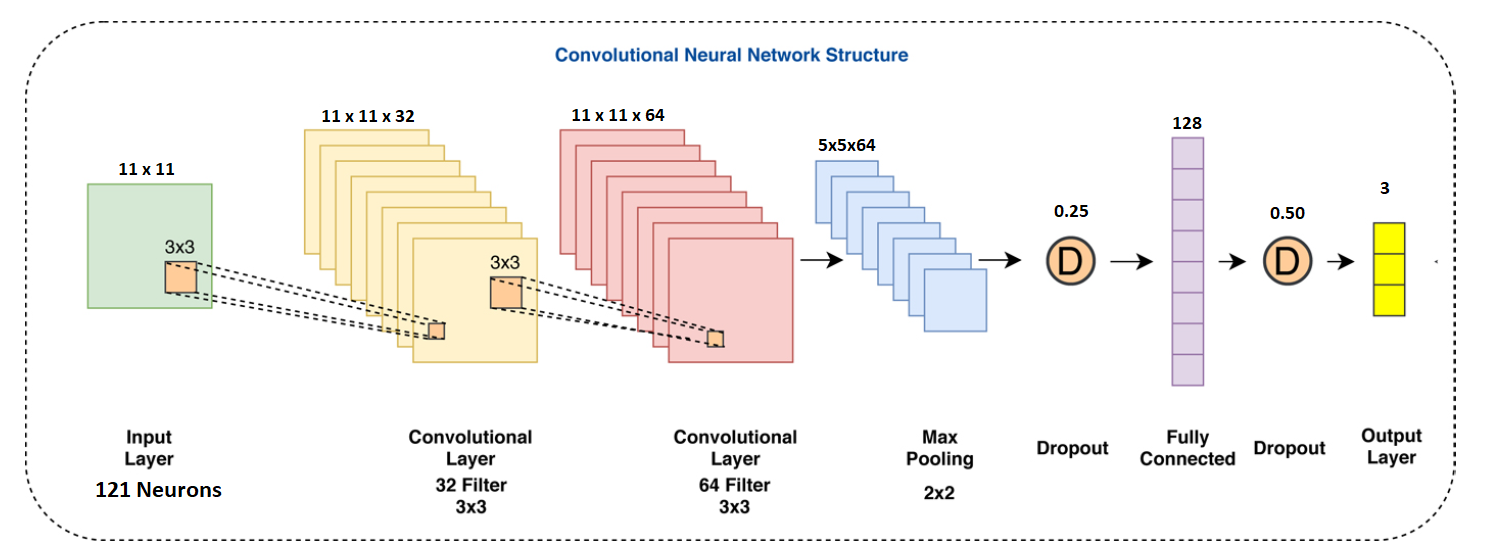
\includegraphics[scale=0.24]{assets/structures/cnn.png}
   \caption{Convolutional Neural Network Structure}
\end{center}
\end{figure}
\noindent
By using an image filter in the convolution layer, we enlarge the channel of the image with stride and padding operations. The filter is generally chosen as 3x3, 5x5 or 7x7. We thought that as the size of the image decreases, the smaller the filter will yield better results as it will enable the image to be scanned more. That's why we chose the filter 3x3. In this way, when we apply 2 convolution layers on the 11x11 image, we get an 11x11x64 image. Then we pass it through the max pooling layer, and we get a 5x5x64 image. Dropout layers are added to prevent overfitting. By reducing the final image to one dimension, we get 128 fully connected neural networks. Then we transform these neural networks into our class labels \textbf{Buy}, \textbf{Hold} \& \textbf{Sell} outputs on the output layer.\vspace{0.1cm} \\*
We used PyTorch while implementing CNN. We selected the hyperparameters based on the best result by training the images with different values. We chose the epoch as 200, the learning rate as 0.001 and the batch size as 64.\vspace{0.3cm} \\*
\textbf{\large ConvMixer}
\begin{figure}[H]
\begin{center}
    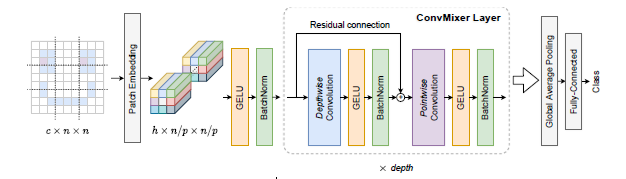
\includegraphics[scale=0.7]{assets/structures/convmixer.png}
    \caption{ConvMixer Structure}
\end{center}
\end{figure}
\noindent
In ConvMixer, we first split the image into patches by applying patch embedding. Then, we pass each patch through the GELU [\textit{Equation 1}] and Batch Normalization [\textit{Equation 2}] layers separately as an activation function. We pass the resulting patches through the ConvMixer layer. The ConvMixer layer contains Depthwise Convolution, activation function, Pointwise Convolution and activation function, respectively. Depthwise Convolution is a sort of convolution in which each input channel receives a single convolutional filter and Pointwise Convolution is a form of convolution that uses a 1x1 kernel, which iterates through each point.\vspace{0.2cm}\\*
We used tensorflow and keras while implementing ConvMixer. In order to select the hyperparameters optimally, we trained the images by giving different numbers of epoch, batch size, patch size, kernel size and learning rate. As a result, we gave the 200 epoch, the batch size 128, the patch size 1, the kernel size 3 and the learning rate 0.01.\vspace{0.2cm} \\*
\textit{Equation 1:} $GELU(x)=xP(X \leq x)=x \phi (x)$ \vspace{0.1cm}\\*
\textit{Equation 2:} $y = ((x - E[x])/\sqrt{Var[x]+\epsilon}) \hspace{0.1cm} \DeclareMathSymbol{*} \hspace{0.1cm} \gamma + \beta$ \vspace{0.3cm} \\*
\textbf{\large Vision Transformer} \\*
\begin{figure}[H]
\begin{center}
    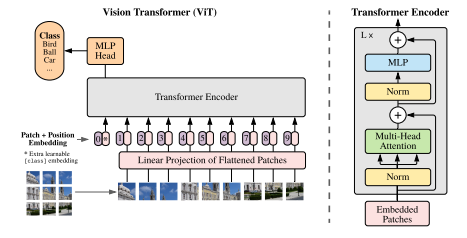
\includegraphics[scale=0.4]{assets/structures/visionTransformer.png}
    \caption{Vision Transformer Structure}
\end{center}
\end{figure}
\noindent
In the Visual Transformer model, the normal transformer model is adapted to the images. 2D images are converted into sequence of flattened 2D patches using patch + position embedding. Then these patches are given to the transformer encoder according to their positions. Transformer Encoder contains 3 layers, these layers are Normalization, Multi-Head Attention, Normalization. Multi-Head Attention is an attention mechanism module that runs through an attention mechanism multiple times in parallel. After the patches pass through these layers, a classification model, MLP, has been added for the classification to take place. We used tensorflow and keras while implementing Vision Transformer. We gave hyperparameters epoch 200, batch size 128, patch size 2 and learning rate 0.001.
\subsection{Technical, Operational \& Financial Feasibility}
\textbf{Technical Feasibility} \vspace{0.1}\\*
We could not use Nvidia CUDA on some architectures since these architectures do not support the current version of TensorFlow, in this case, we ran the code on the CPU instead of the GPU, which increased the code's runtime, but when we used Nvidia CUDA in the CNN architecture, the code's runtime decreased by 1 quarter.\vspace{0.2cm}\\*
\textbf{Financial Feasibility} \vspace{0.1}\\*
We don't have any other cost without needing a better performing and equipped computer to train our model.
\subsection{Knowledge \& Skill Set}
Different skill sets from various courses were used in this project. While the courses mentioned here had the most impact on our project, all the CS courses we've reviewed so far have given us new perspectives in implementing this project.\vspace{0.2cm} \\*
\textbf{CS 101:} The basics of programming were learned and helped to use the basic knowledge in this project.\vspace{0.1cm} \\*
\textbf{CS 320:} Helped us to design and write the project reports accurately.\vspace{0.1cm}\\*
\textbf{CS 447:} Helped us to request Yahoo Finance data. \vspace{0.1cm}\\*
\textbf{CS 452:} Helped us to create and pre-process the dataset as well as apply the classification model. \vspace{0.1cm}\\*
\textbf{CS 454:} Helped us to understand the neural network logic and its pros and cons. \vspace{0.1cm}\\*
\textbf{MATH 211:} Helped us to understand the matrices in the structure of the images. \vspace{0.1cm} \\*
\textbf{MATH 217:} Help us to compare statistics in results.
\subsection{Engineering Standards}
• Style Guide for Python Code\\*
• Data Format: NumPy Array\\*
• HTTP Protocols: GET

\begin{center}
    \item\section{Results and Discussion}
\end{center}
We attempted to obtain results with the ConvMixer and Vision Transformer architectures using the dataset we generated. These results, as well as a comparison to the CNN-TA article's results, are shown below. \vspace{0.2cm}\\*
To begin with, one of the most significant findings was that the distribution of predictions in the ConvMixer architecture was more diversified than that of the Vision Transformer architecture. The ConvMixer model assessed the buy points more accurately than the Vision Transformer model, as demonstrated by the confusion matrices in Table 1 and Table 3. While the Vision Transformer model performed better in hold predictions, both models accurately identified 18 pictures in sell. Because 49.8 percent of our dataset is labeled hold, a model is more likely to predict hold correctly. Therefore, the fact that the ConvMixer model has a better prediction percentage than the Vision Transformer for buy labeled images may indicate that the ConvMixer model is more resistant to imbalanced datasets.

\begin{table}[H]
    \centering
    \caption{Confusion Matrix of ConvMixer}
    \begin{tabular}{llcccll}
        \cline{1-5}
        \multicolumn{1}{|l|}{} & \multicolumn{1}{l|}{} & \multicolumn{3}{c|}{Predicted} & & \\\cline{1-5} \multicolumn{1}{|l|}{} & \multicolumn{1}{l|}{} & \multicolumn{1}{l|}{Buy} & \multicolumn{1}{l|}{Hold} & \multicolumn{1}{l|}{Sell} & & \\ \cline{1-5} \multicolumn{1}{|c|}{\multirow{3}{*}{Actual}} & \multicolumn{1}{l|}{Buy} & \multicolumn{1}{c|}{40} & \multicolumn{1}{c|}{73} & \multicolumn{1}{c|}{22} & & \\ \cline{2-5} \multicolumn{1}{|c|}{} & \multicolumn{1}{l|}{Hold} & \multicolumn{1}{c|}{30} & \multicolumn{1}{c|}{204}  & \multicolumn{1}{c|}{14}& & \\ \cline{2-5} \multicolumn{1}{|c|}{} & \multicolumn{1}{l|}{Sell} & \multicolumn{1}{c|}{29} & \multicolumn{1}{c|}{66} & \multicolumn{1}{c|}{18} & & \\ \cline{1-5} & & \multicolumn{1}{l}{} & \multicolumn{1}{l}{} & \multicolumn{1}{l}{} &&
    \end{tabular}
\end{table}
\begin{table}[H]
    \centering
    \caption{Classification Report of ConvMixer}
    \begin{tabular}{lcccll}
        \cline{1-4}
        \multicolumn{4}{|c|}{\textbf{Total Accuracy: 0.53}} & & \\\cline{1-4} \multicolumn{1}{|l|}{} & \multicolumn{1}{l|}{Buy} & \multicolumn{1}{l|}{Hold} & \multicolumn{1}{l|}{Sell} & & \\\cline{1-4} \multicolumn{1}{|l|}{Recall} & \multicolumn{1}{c|}{0.30} & \multicolumn{1}{c|}{0.82} & \multicolumn{1}{c|}{0.16} & & \\\cline{1-4} \multicolumn{1}{|l|}{Precision} & \multicolumn{1}{c|}{0.40} & \multicolumn{1}{c|}{0.59} & \multicolumn{1}{c|}{0.33} & &  \\\cline{1-4} \multicolumn{1}{|l|}{F1 Score} & \multicolumn{1}{c|}{0.34} & \multicolumn{1}{c|}{0.69} & \multicolumn{1}{c|}{0.22} & &  \\\cline{1-4} & \multicolumn{1}{l}{} & \multicolumn{1}{l}{} & \multicolumn{1}{l}{} & & 
    \end{tabular}
\end{table}
\begin{table}[H]
    \centering
    \caption{Confusion Matrix of Vision Transformer}
    \begin{tabular}{llcccll}
        \cline{1-5}
        \multicolumn{1}{|l|}{} & \multicolumn{1}{l|}{} & \multicolumn{3}{c|}{Predicted} & & \\\cline{1-5} \multicolumn{1}{|l|}{} & \multicolumn{1}{l|}{} & \multicolumn{1}{l|}{Buy} & \multicolumn{1}{l|}{Hold} & \multicolumn{1}{l|}{Sell} & & \\\cline{1-5} \multicolumn{1}{|c|}{\multirow{3}{*}{Actual}} & \multicolumn{1}{l|}{Buy} & \multicolumn{1}{c|}{12} & \multicolumn{1}{c|}{103} & \multicolumn{1}{c|}{20} & & \\\cline{2-5} \multicolumn{1}{|c|}{} & \multicolumn{1}{l|}{Hold} & \multicolumn{1}{c|}{1} & \multicolumn{1}{c|}{234} & \multicolumn{1}{c|}{13} & & \\\cline{2-5} \multicolumn{1}{|c|}{} & \multicolumn{1}{l|}{Sell} & \multicolumn{1}{c|}{8} & \multicolumn{1}{c|}{87} & \multicolumn{1}{c|}{18} & & \\\cline{1-5} & & \multicolumn{1}{l}{} & \multicolumn{1}{l}{} & \multicolumn{1}{l}{} & & 
    \end{tabular}
\end{table}
\begin{table}[H]
    \centering
    \caption{Classification Report of Vision Transformer}
    \begin{tabular}{lcccll}
        \cline{1-4}
        \multicolumn{4}{|c|}{\textbf{Total Accuracy: 0.53}} & & \\\cline{1-4} \multicolumn{1}{|l|}{} & \multicolumn{1}{l|}{Buy} & \multicolumn{1}{l|}{Hold} & \multicolumn{1}{l|}{Sell} & & \\ \cline{1-4} \multicolumn{1}{|l|}{Recall} & \multicolumn{1}{c|}{0.09} & \multicolumn{1}{c|}{0.94} & \multicolumn{1}{c|}{0.16} & & \\\cline{1-4} \multicolumn{1}{|l|}{Precision} & \multicolumn{1}{c|}{0.57} & \multicolumn{1}{c|}{0.55} & \multicolumn{1}{c|}{0.35} & & \\\cline{1-4} \multicolumn{1}{|l|}{F1 Score} & \multicolumn{1}{c|}{0.15} & \multicolumn{1}{c|}{0.70} & \multicolumn{1}{c|}{0.22} & & \\\cline{1-4} & \multicolumn{1}{l}{} & \multicolumn{1}{l}{} & \multicolumn{1}{l}{} & &
    \end{tabular}
\end{table}
\noindent
In Table 5, it is seen that 89.9 percent of the test datasets are labeled as hold. This demonstrates that the dataset used for CNN-TA is much more imbalanced than our dataset. In addition, while the CNN-TA model was evaluated with 33714 test data, the test data we used to evaluate our ConvMixer and Vision Transformer models consisted of 496 images. This may explain why the total accuracy of our models is lower than that of CNN-TA and why both models are subject to overfitting very quickly.
\begin{table}[H]
    \centering
    \caption{Confusion Matrix of CNN-TA}
    \begin{tabular}{llcccll}
        \cline{1-5}
        \multicolumn{1}{|l|}{} & \multicolumn{1}{l|}{} & \multicolumn{3}{c|}{Predicted} & & \\\cline{1-5} \multicolumn{1}{|l|}{} & \multicolumn{1}{l|}{} & \multicolumn{1}{l|}{Buy} & \multicolumn{1}{l|}{Hold} & \multicolumn{1}{l|}{Sell} & & \\\cline{1-5} \multicolumn{1}{|c|}{\multirow{3}{*}{Actual}} & \multicolumn{1}{l|}{Buy} & \multicolumn{1}{c|}{1215} & \multicolumn{1}{c|}{478} & \multicolumn{1}{c|}{0} & & \\\cline{2-5} \multicolumn{1}{|c|}{} & \multicolumn{1}{l|}{Hold} & \multicolumn{1}{c|}{5180} & \multicolumn{1}{c|}{18629} & \multicolumn{1}{c|}{6498} & & \\\cline{2-5} \multicolumn{1}{|c|}{} & \multicolumn{1}{l|}{Sell} & \multicolumn{1}{c|}{0} & \multicolumn{1}{c|}{587} & \multicolumn{1}{c|}{1127} & & \\\cline{1-5} & & \multicolumn{1}{l}{} & \multicolumn{1}{l}{} & \multicolumn{1}{l}{} & & 
    \end{tabular}
\end{table}
\begin{table}[H]
    \centering
    \caption{Classification Report of CNN-TA}
    \begin{tabular}{lcccll}
        \cline{1-4}
        \multicolumn{4}{|c|}{\textbf{Total Accuracy: 0.62}} & & \\\cline{1-4} \multicolumn{1}{|l|}{} & \multicolumn{1}{l|}{Buy} & \multicolumn{1}{l|}{Hold} & \multicolumn{1}{l|}{Sell} & & \\ \cline{1-4} \multicolumn{1}{|l|}{Recall} & \multicolumn{1}{c|}{0.72} & \multicolumn{1}{c|}{0.61} & \multicolumn{1}{c|}{0.66} & & \\\cline{1-4} \multicolumn{1}{|l|}{Precision} & \multicolumn{1}{c|}{0.19} & \multicolumn{1}{c|}{0.95} & \multicolumn{1}{c|}{0.15} &  &  \\\cline{1-4} \multicolumn{1}{|l|}{F1 Score}  & \multicolumn{1}{c|}{0.30} & \multicolumn{1}{c|}{0.75} & \multicolumn{1}{c|}{0.24} & & \\\cline{1-4} & \multicolumn{1}{l}{} & \multicolumn{1}{l}{} & \multicolumn{1}{l}{} & &
    \end{tabular}
\end{table}
\noindent
In addition, as mentioned above, the size of the dataset we prepared was considerably smaller than the size of the dataset prepared for the CNN-TA model. This may have caused our models to experience rapid overfitting. In order to minimize overfitting, we plan to increase the number of data points and perform cross-validation in the future. \vspace{0.2cm}\\*
\textbf{\large Model Accuracy \& Loss Graph of ConvMixer}
\begin{figure}[H]
    \begin{center}
        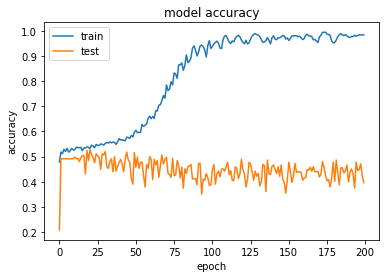
\includegraphics[scale=0.6]{assets/graphs/accuracy_convmixer.png}
        \caption{Train - Test Accuracy Graph}
    \end{center}
\end{figure}
\begin{figure}[H]
    \begin{center}
        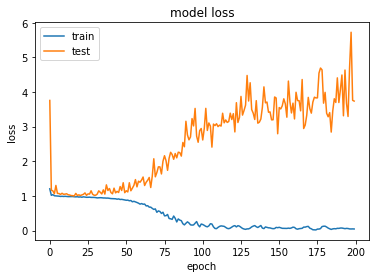
\includegraphics[scale=0.6]{assets/graphs/loss_convmixer.png}
        \caption{Train - Test Loss Graph}
    \end{center}
\end{figure}
\vspace{1.38cm}
\textbf{\large Model Accuracy \& Loss Graph of Vision Transform}
\begin{figure}[H]
    \begin{center}
        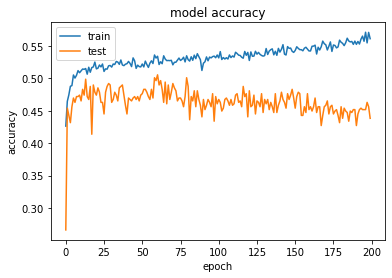
\includegraphics[scale=0.6]{assets/graphs/accuracy_vt.png}
        \caption{Train - Test Accuracy Graph}
    \end{center}
\end{figure}
\begin{figure}[H]
    \begin{center}
        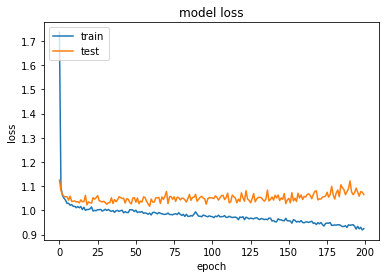
\includegraphics[scale=0.6]{assets/graphs/loss_vt.png}
        \caption{Train - Test Loss Graph}
    \end{center}
\end{figure}
\noindent
We also tried to implement the CNN-TA architecture using PyTorch and train it with our own dataset, but we could not obtain results that we can graph. Within the scope of CS402, we plan to add this to the models we develop and compare.\vspace{0.2cm} \\*
Moreover, all models were trained on an Intel i7 4510-U CPU. That's why we had to limit the amount of data we collected. \newline
As the project progresses, we intend to train our models with GPUs on a platform such as Azure, AWS Cloud, or Google Cloud.

\begin{center}
    \item\section{Related Work}
\end{center}
In many academic studies, machine learning models were used when stock prediction was made because stock prices are time series data. Nevertheless, the machine learning models used for stock-price prediction were not performing excellently. Thus, better-performing models were required for stock prices.\vspace{0.2cm} \\*
In recent years, forecast models based on deep learning have emerged as the best performers in financial forecasts. Moreover, many academic and sectoral studies have been conducted using different deep-learning models. The article named "Attention Augmented Convolutional Networks" [1] implemented by the Google Brain team under the umbrella of Google AI, the article named "Algorithmic Financial Trading with Deep Convolutional Neural Networks: Time Series to Image Conversion Approach" [2], the article named "Patches Are All You Need?" [3] or the article named "An Image is Worth 16x16 Words: Transformers for Image Recognition at Scale" [4] can be given examples of these studies. Our approach in the senior project is analogous to the "Algorithmic Financial Trading with Deep Convolutional Neural Networks: Time Series to Image Conversion Approach" article, but while using Convolutional Neural Network (CNN) in this article, we use the ConvMixer architecture, introduced in 2021, which is thought to perform better according to research's.\vspace{0.2cm} \\*
Although CNNs have dominated computer vision tasks for many years, recent research has shown that Transformer-based models, most notably the Vision Transformer (ViT), can outperform CNN in some cases.[3] ConvMixer an extremely straightforward model that is similar to the ViT; hence, we are using this architecture in our senior project.

\begin{center}
    \item\section{Conclusion and Future Work}
\end{center}
In this section, we provide a brief summary of the senior project and we talk about the future work of the project.\\*
\subsection{Conclusion}
To summarize our senior project, we use the ConvMixer model that predicts Stock Price and Direction with the help of Deep Attention Based Convolutional Neural Networks after transforming 1D time-series signal images into 2D time-series signals with the help of technical indicators. We think that the last version of senior project will have a consequential economic impact. \vspace{0.4cm} \\*
Companies or investors can buy their stocks in a more optimized way with the last version of our senior project, and as a result, investors can use the money that normally is melt away by their manual trading techniques on different opportunities. Furthermore, We think that our project will have an optimistic social impact because we believe that investors can be mirthful with the right investments they make. Also, After some thought about what ethical issues we might encounter in our senior project, we realized that there might be a problem. If the model we will apply constructs an inaccurate prediction, we can mislead the investors \& companies and make an erroneous investment decision.
\subsection{Future Work}
• Finding the best hyperparameters of our model using sites like Weights \& Biases. [5]\\*
• Utilizing the Cross-Validation to make the performance of the model more accurate.\\*
• On a high-dimensional scale, the assessment measures and their correlation may be examined.\\*
• Running models on different Datasets \& Technical Indicators and reporting the results.\\*
• Testing the model on a major crypto exchange platform like Binance after doing the work above.\\*
• Finally, implementing a new project that makes an automatic trading bot for cryptocurrencies using this model.

\begin{center}
    \textbf{\Large Acknowledgements}
\end{center}
For his support and advice throughout our senior project, we would like to express our thanks and gratitude to our advisor Assistant Prof. Emre Sefer.

\begin{center}
    \textbf{\Large References}
\end{center}
[1] Bello, I., Zoph, B., Vaswani, A., Shlens, J., &amp; Le, Q. V. (2020, September 9). Attention augmented convolutional networks. arXiv.org. Retrieved January 4, 2022, from \href{https://arxiv.org/abs/1904.09925}{https://arxiv.org/abs/1904.09925}\vspace{0.1cm} \newline
[2] Sezer, O. B., &amp; Ozbayoglu, A. M. (2018, April 27). Algorithmic financial trading with deep convolutional neural networks: Time Series to Image Conversion Approach. Applied Soft Computing. Retrieved January 4, 2022, from \href{https://www.sciencedirect.com/science/article/abs/pii/S1568494618302151}{https://www.sciencedirect.com/science/article/abs/pii/S1568494618302151}\vspace{0.1cm} \newline
[3] Anonymous. (2021, November 23). Patches are all you need? OpenReview. Retrieved January 5, 2022, from \href{https://openreview.net/forum?id=TVHS5Y4dNvM}{https://openreview.net/forum?id=TVHS5Y4dNvM}\vspace{0.1cm} \newline
[4] Dosovitskiy, A., Beyer, L., Kolesnikov, A., Weissenborn, D., Zhai, X., Unterthiner, T., Dehghani, M., Minderer, M., Heigold, G., Gelly, S., Uszkoreit, J., &amp; Houlsby, N. (2021, June 3). An image is worth 16x16 words: Transformers for image recognition at scale. arXiv.org. Retrieved January 5, 2022, from \href{https://arxiv.org/abs/2010.11929}{https://arxiv.org/abs/2010.11929} \vspace{0.1cm} \newline
[5] Weights &amp; Biases – developer tools for ML. Weights &amp; Biases – Developer tools for ML. (n.d.). Retrieved January 5, 2022, from \href{https://wandb.ai/site}{https://wandb.ai/site} \vspace{0.1cm} \newline

\begin{center}
    \textbf{\Large Appendix}
\end{center}
\begin{figure}[H]
\begin{center}
    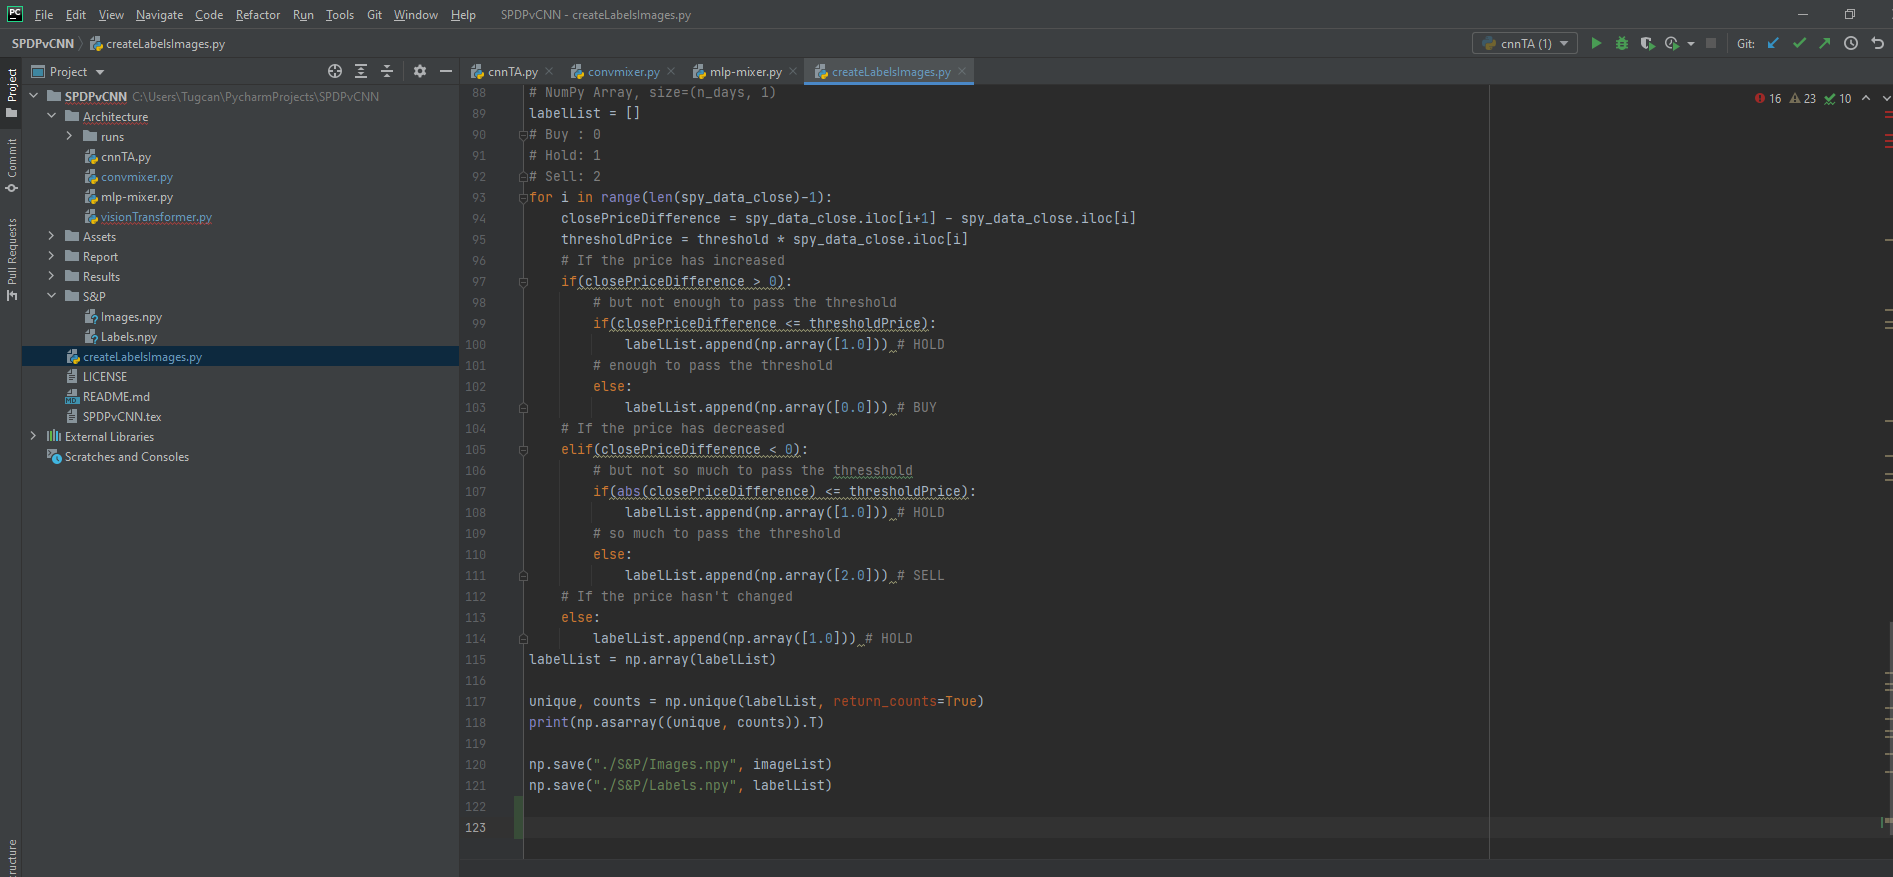
\includegraphics[scale=0.18]{assets/appendix/image_creation_alg.png}
    \caption{Algorithm of Labeling}
\end{center}
\end{figure}
\noindent
\begin{figure}[H]
\begin{center}
    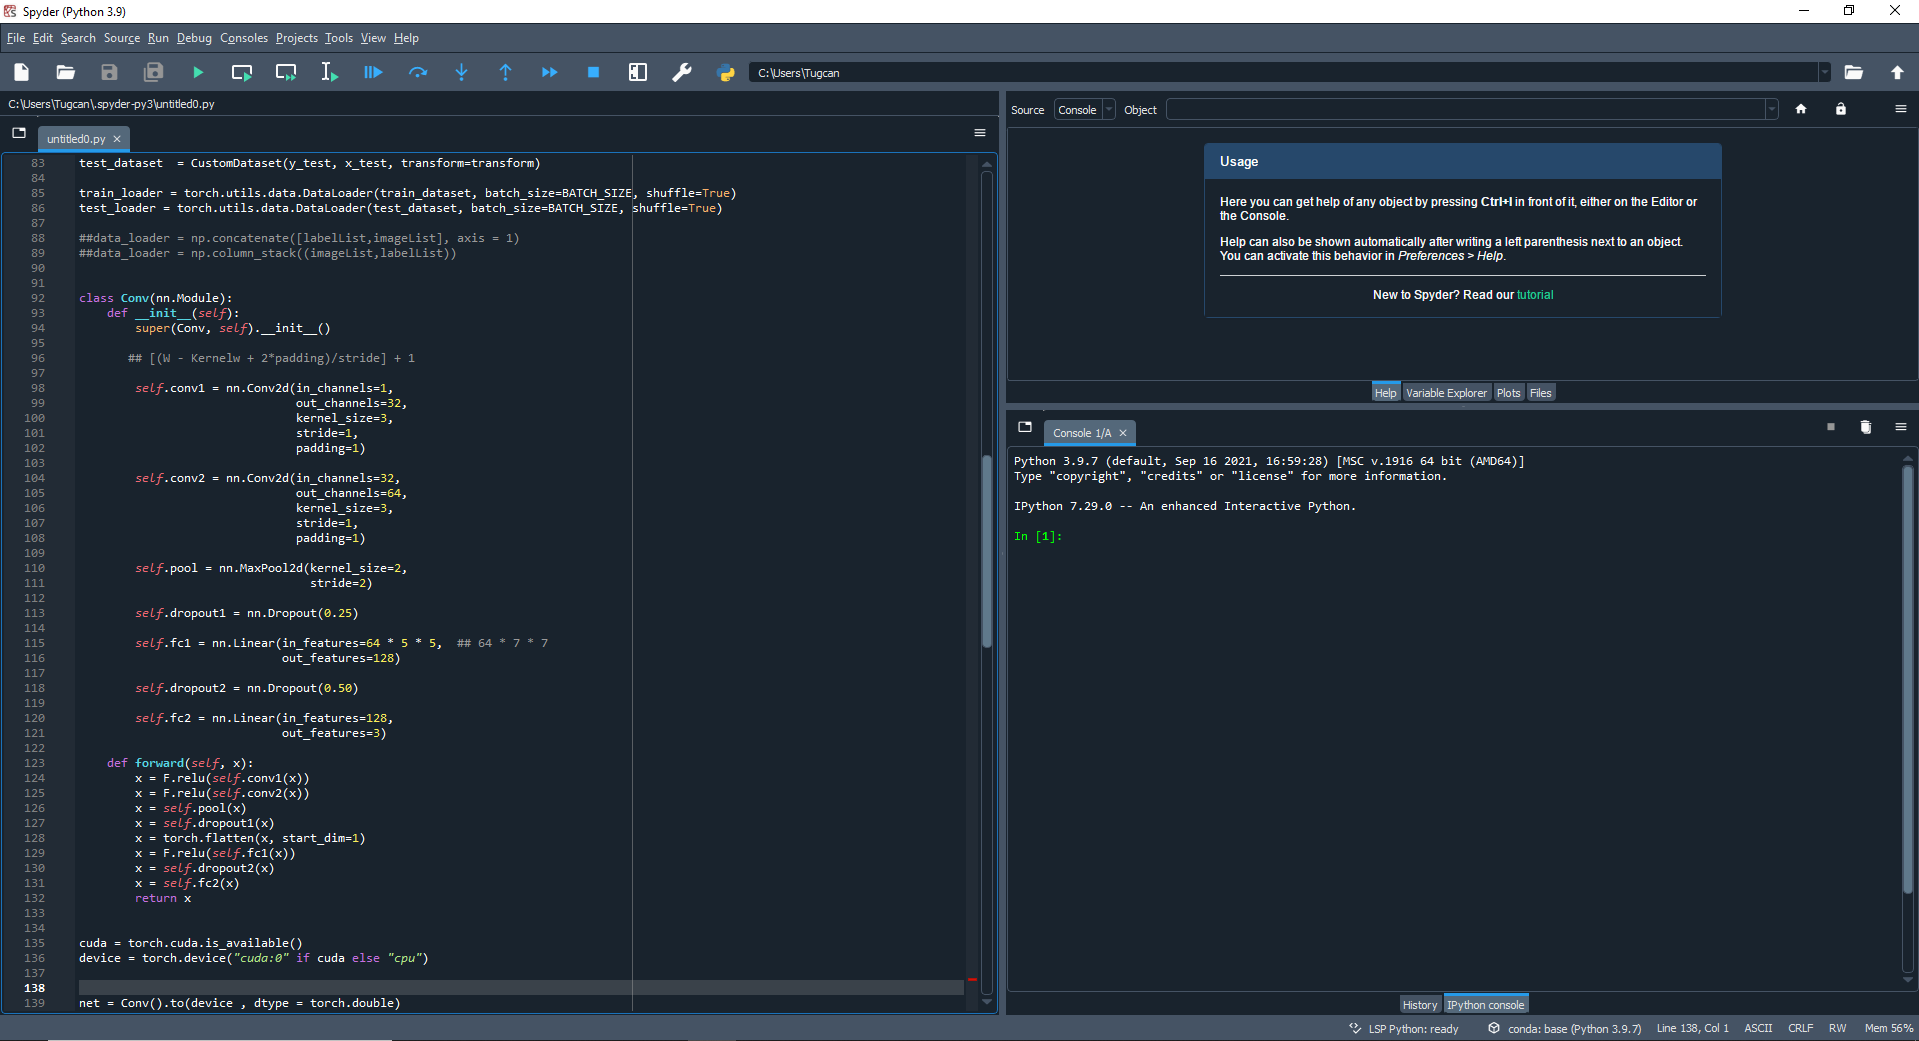
\includegraphics[scale=0.18]{assets/appendix/cnn_implemantation.png}
    \caption{Algorithm of Convolutional Neural Network}
\end{center}
\end{figure}
\noindent
\begin{figure}[H]
\begin{center}
    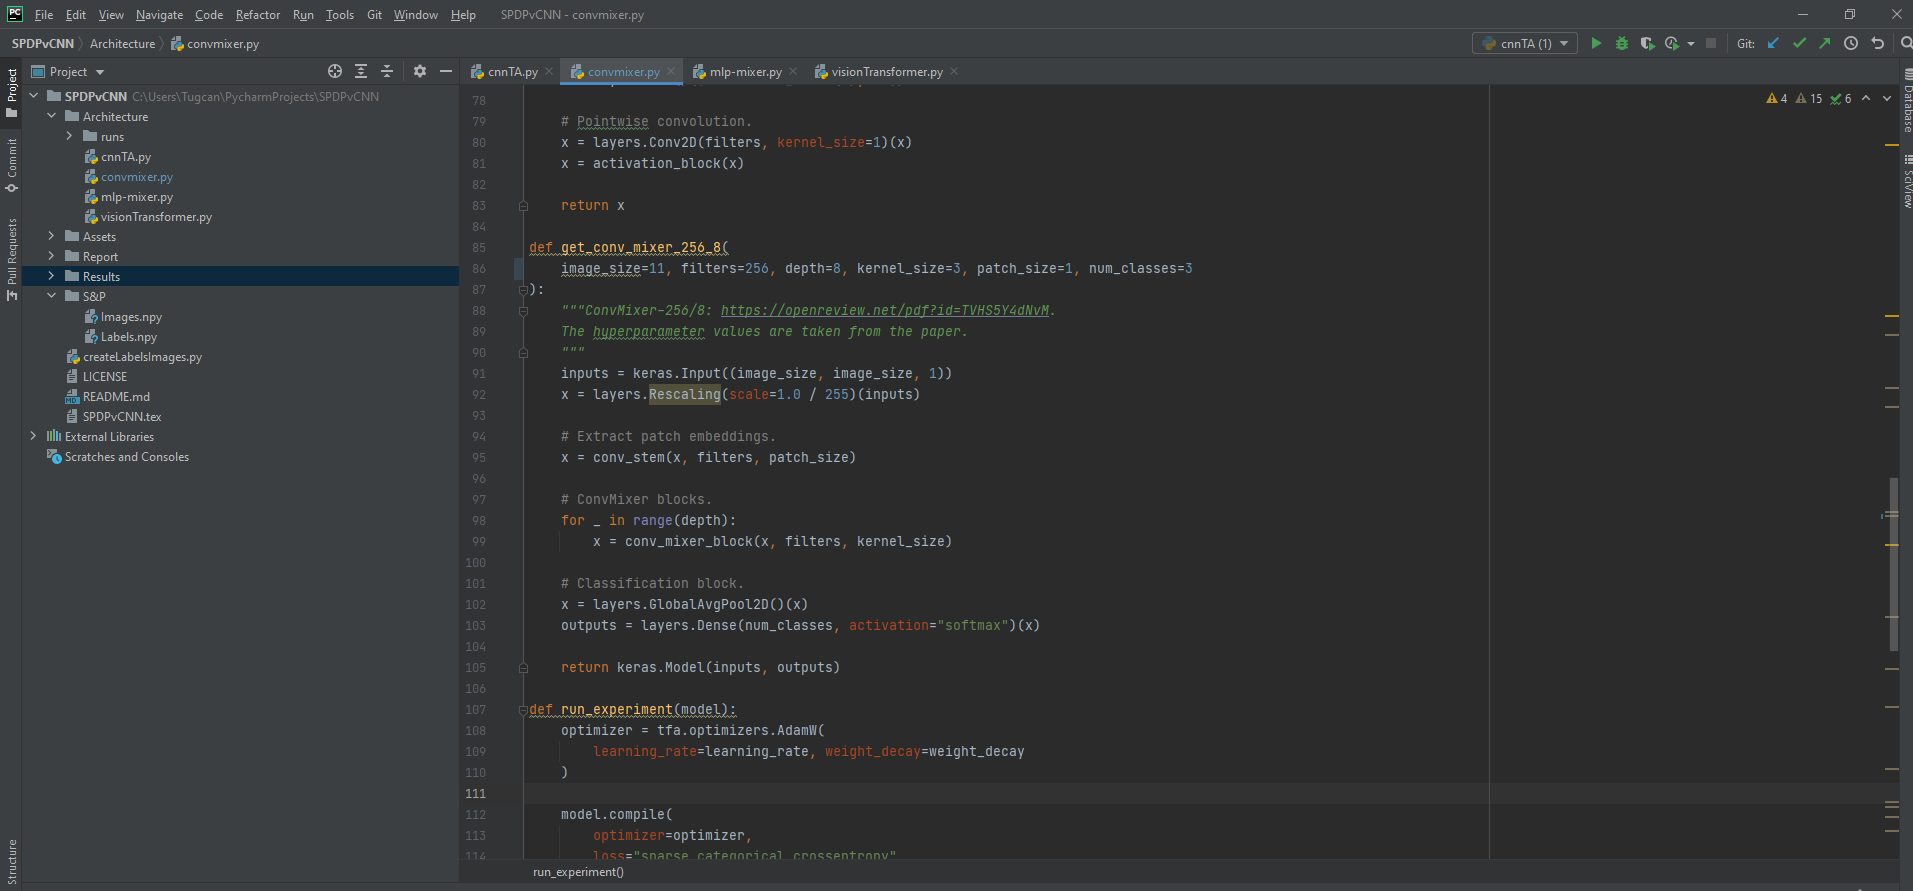
\includegraphics[scale=0.18]{assets/appendix/convmixer_implemantation.png}
    \caption{Algorithm of ConvMixer}
\end{center}
\end{figure}
\noindent
\begin{figure}[H]
\begin{center}
    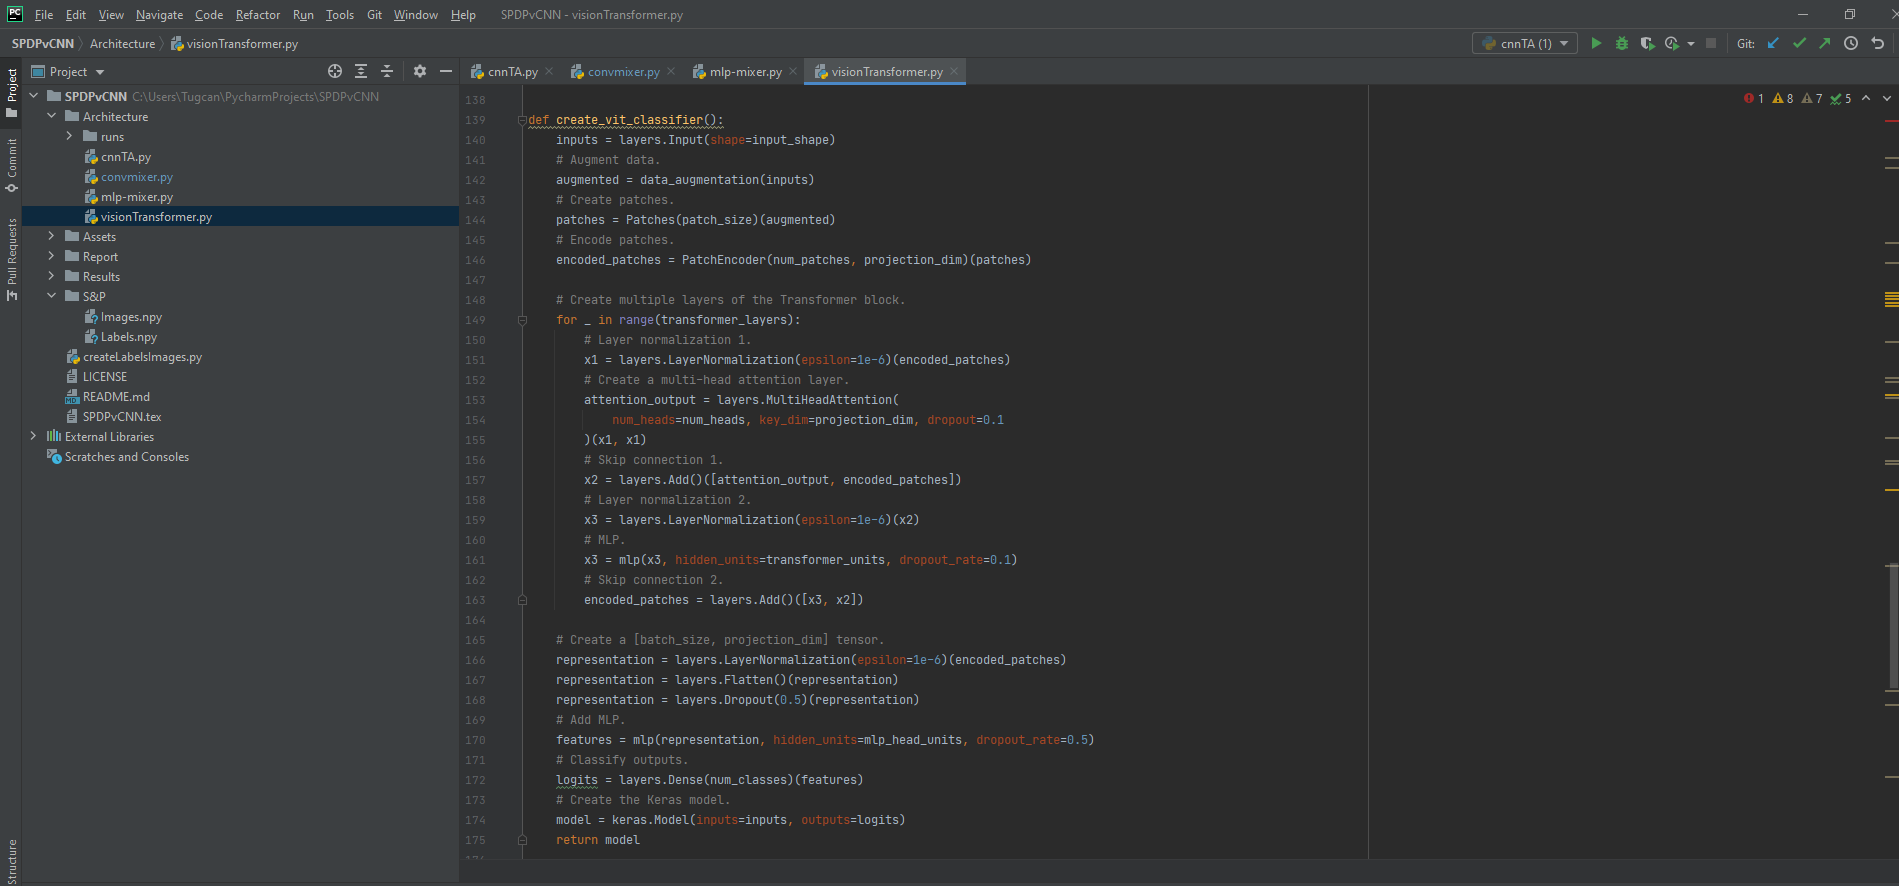
\includegraphics[scale=0.18]{assets/appendix/vit_implemantation.png}
    \caption{Algorithm of Vision Transformer}
\end{center}
\end{figure}
\noindent
\end{document}
